The primary objective of this thesis is to assess the potentials and limitations of a self developed APR pipeline prototype. We aim to answer the following research questions to evaluate the system's capabilities and impact on the software development process:

\begin{itemize}
    \item \textbf{RQ1:} How can LLM-based automated bug fixing be effectively and efficiently integrated into a CI pipeline?
    \item \textbf{RQ2:} What are the key potentials of this integrated approach in terms of repair success rate, cost-effectiveness and developer workflow enhancement?
    \item \textbf{RQ3:} What are the primary limitations and challenges, such as performance overhead, accuracy, and security, of using LLM-based APR within a CI context?
\end{itemize}

For answering these questions we streamlined this process into three phases Preparation, Implementation and Evaluation, shown in Figure \ref{fig:method-overview}.

\begin{figure}[H]
    \centering
    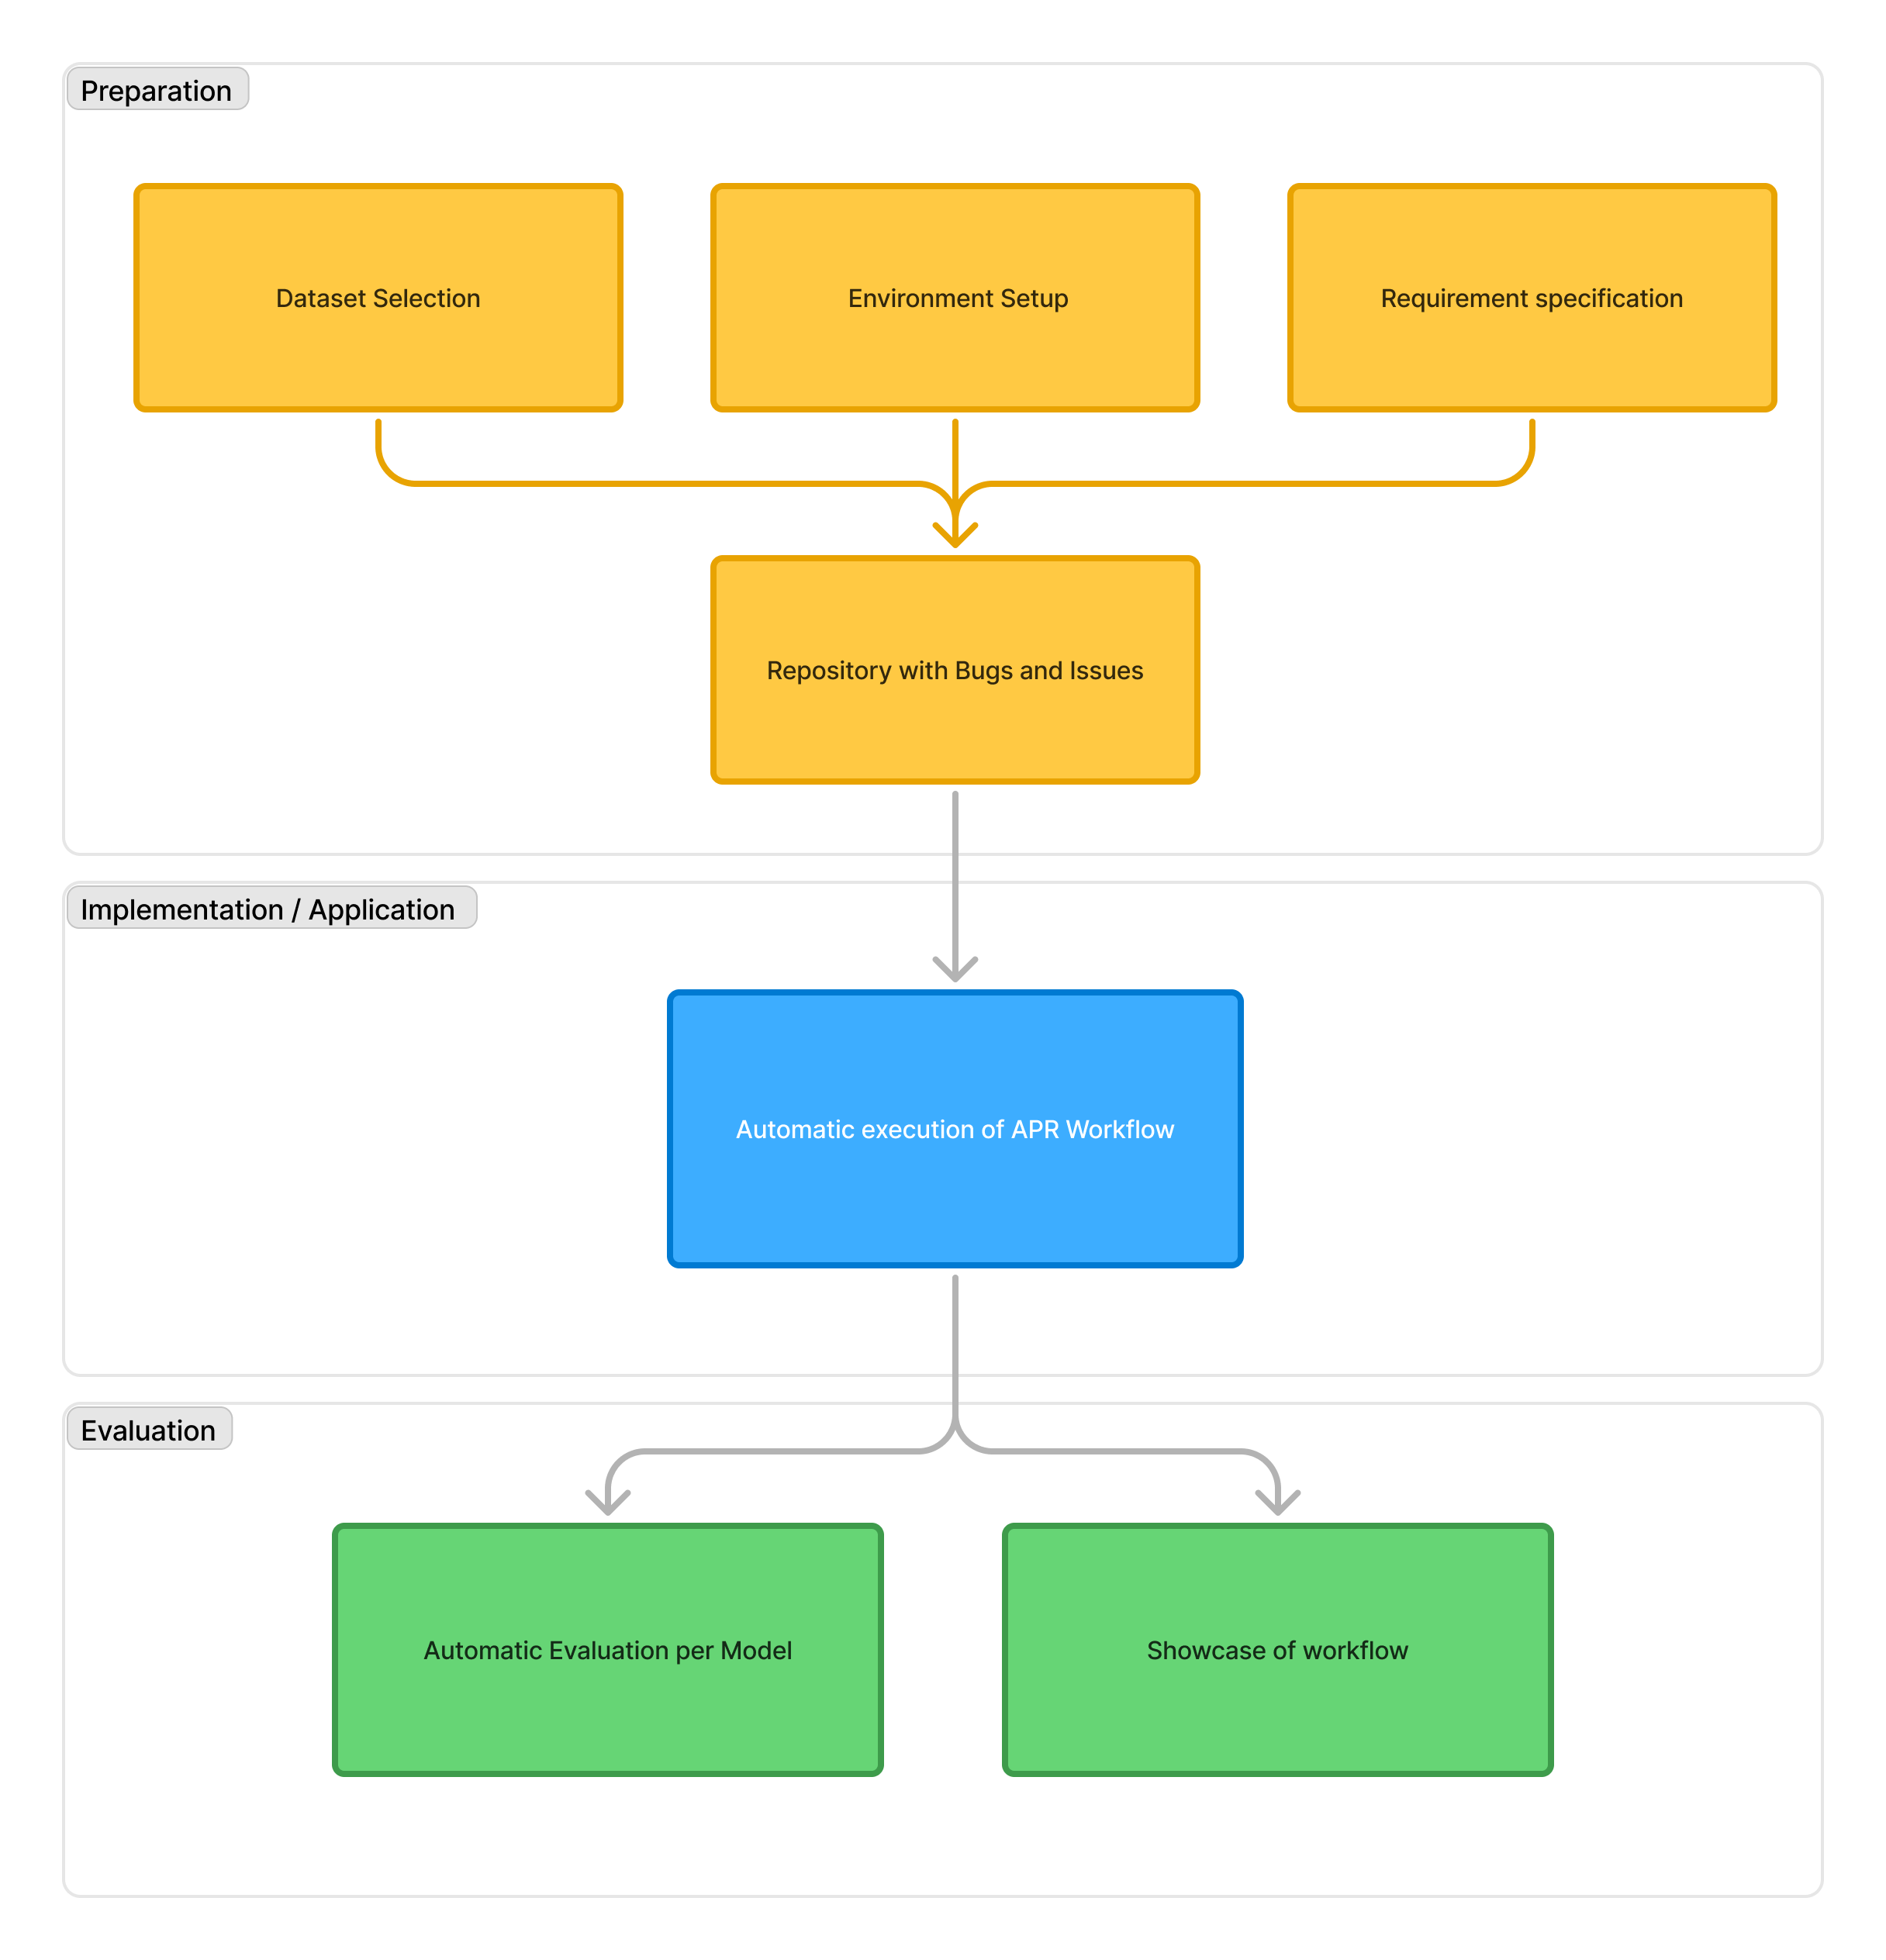
\includegraphics[width=1\textwidth]{images/method.png}
    \caption{Simple Action}
    \label{fig:method-overview}
\end{figure}

In the preparation we select a suitable APR benchmark. With this benchmark we set up a realistic development environment. By specifying requirements we lay the groundwork for the implementation of the APR system.
In the second part we implement the APR system as a GitHub Action workflow based on the requirements.
Lastly evaluation of the self developed prototype is done by using the defined evaluation metrics \ref{section:evaluation} collected during the execution of the APR system. Furthermore we will showcase the resulting workflow of using the system in a repository.
The following sections will go into detail of each of these phases.

\section{Preparation}
For implementing and evaluating our system we first need to prepare an environment where the system can be integrated and used. This includes selecting a suitable dataset, setting up the environment, and specifying the requirements for the system.
\subsection{Dataset Selection}
For the evaluation of our APR integration, we selected the QuixBugs benchmark \cite{linQuixBugsMultilingualProgram2017}. This dataset is well-suited for our purposes due to its focus on small-scale software bugs in Python. It consists of 40 individual files containing an algorithmic bug each. The bug is always caused by single erroneous line. QuixBugs brings corresponding tests and a corrected version for every file which allows for repair validation. The bugs where developed as challenging problems for developers \cite{linQuixBugsMultilingualProgram2017}, it enables us to evaluate if our system can take over the cognitive demanding task of fixing small bugs without developer intervention.

Compared to other APR benchmarks \ref{table:benchmarks} like SWE-Bench \cite{jimenezSWEbenchCanLanguage2024} QuixBugs is relatively small which allows for accelerated setup and development.

\subsection{Environment Setup}
To mirror realistic software development environment, we prepared a GitHub repository containing the QuixBugs datasets python files. This repository serves as the basis for the bug fixing process, allowing the system to interact with the codebase and perform repairs. The repository contains only relevant files and folders required for the bug fixing process, ensuring a clean environment for the system to operate in.

Using the relevant files we generate a GitHub issue for each bug, using a consistent template that captures only the title of the Problem. These issues serve as the entry points and communication medium to our APR pipeline.

\begin{figure}[H]
    \centering
    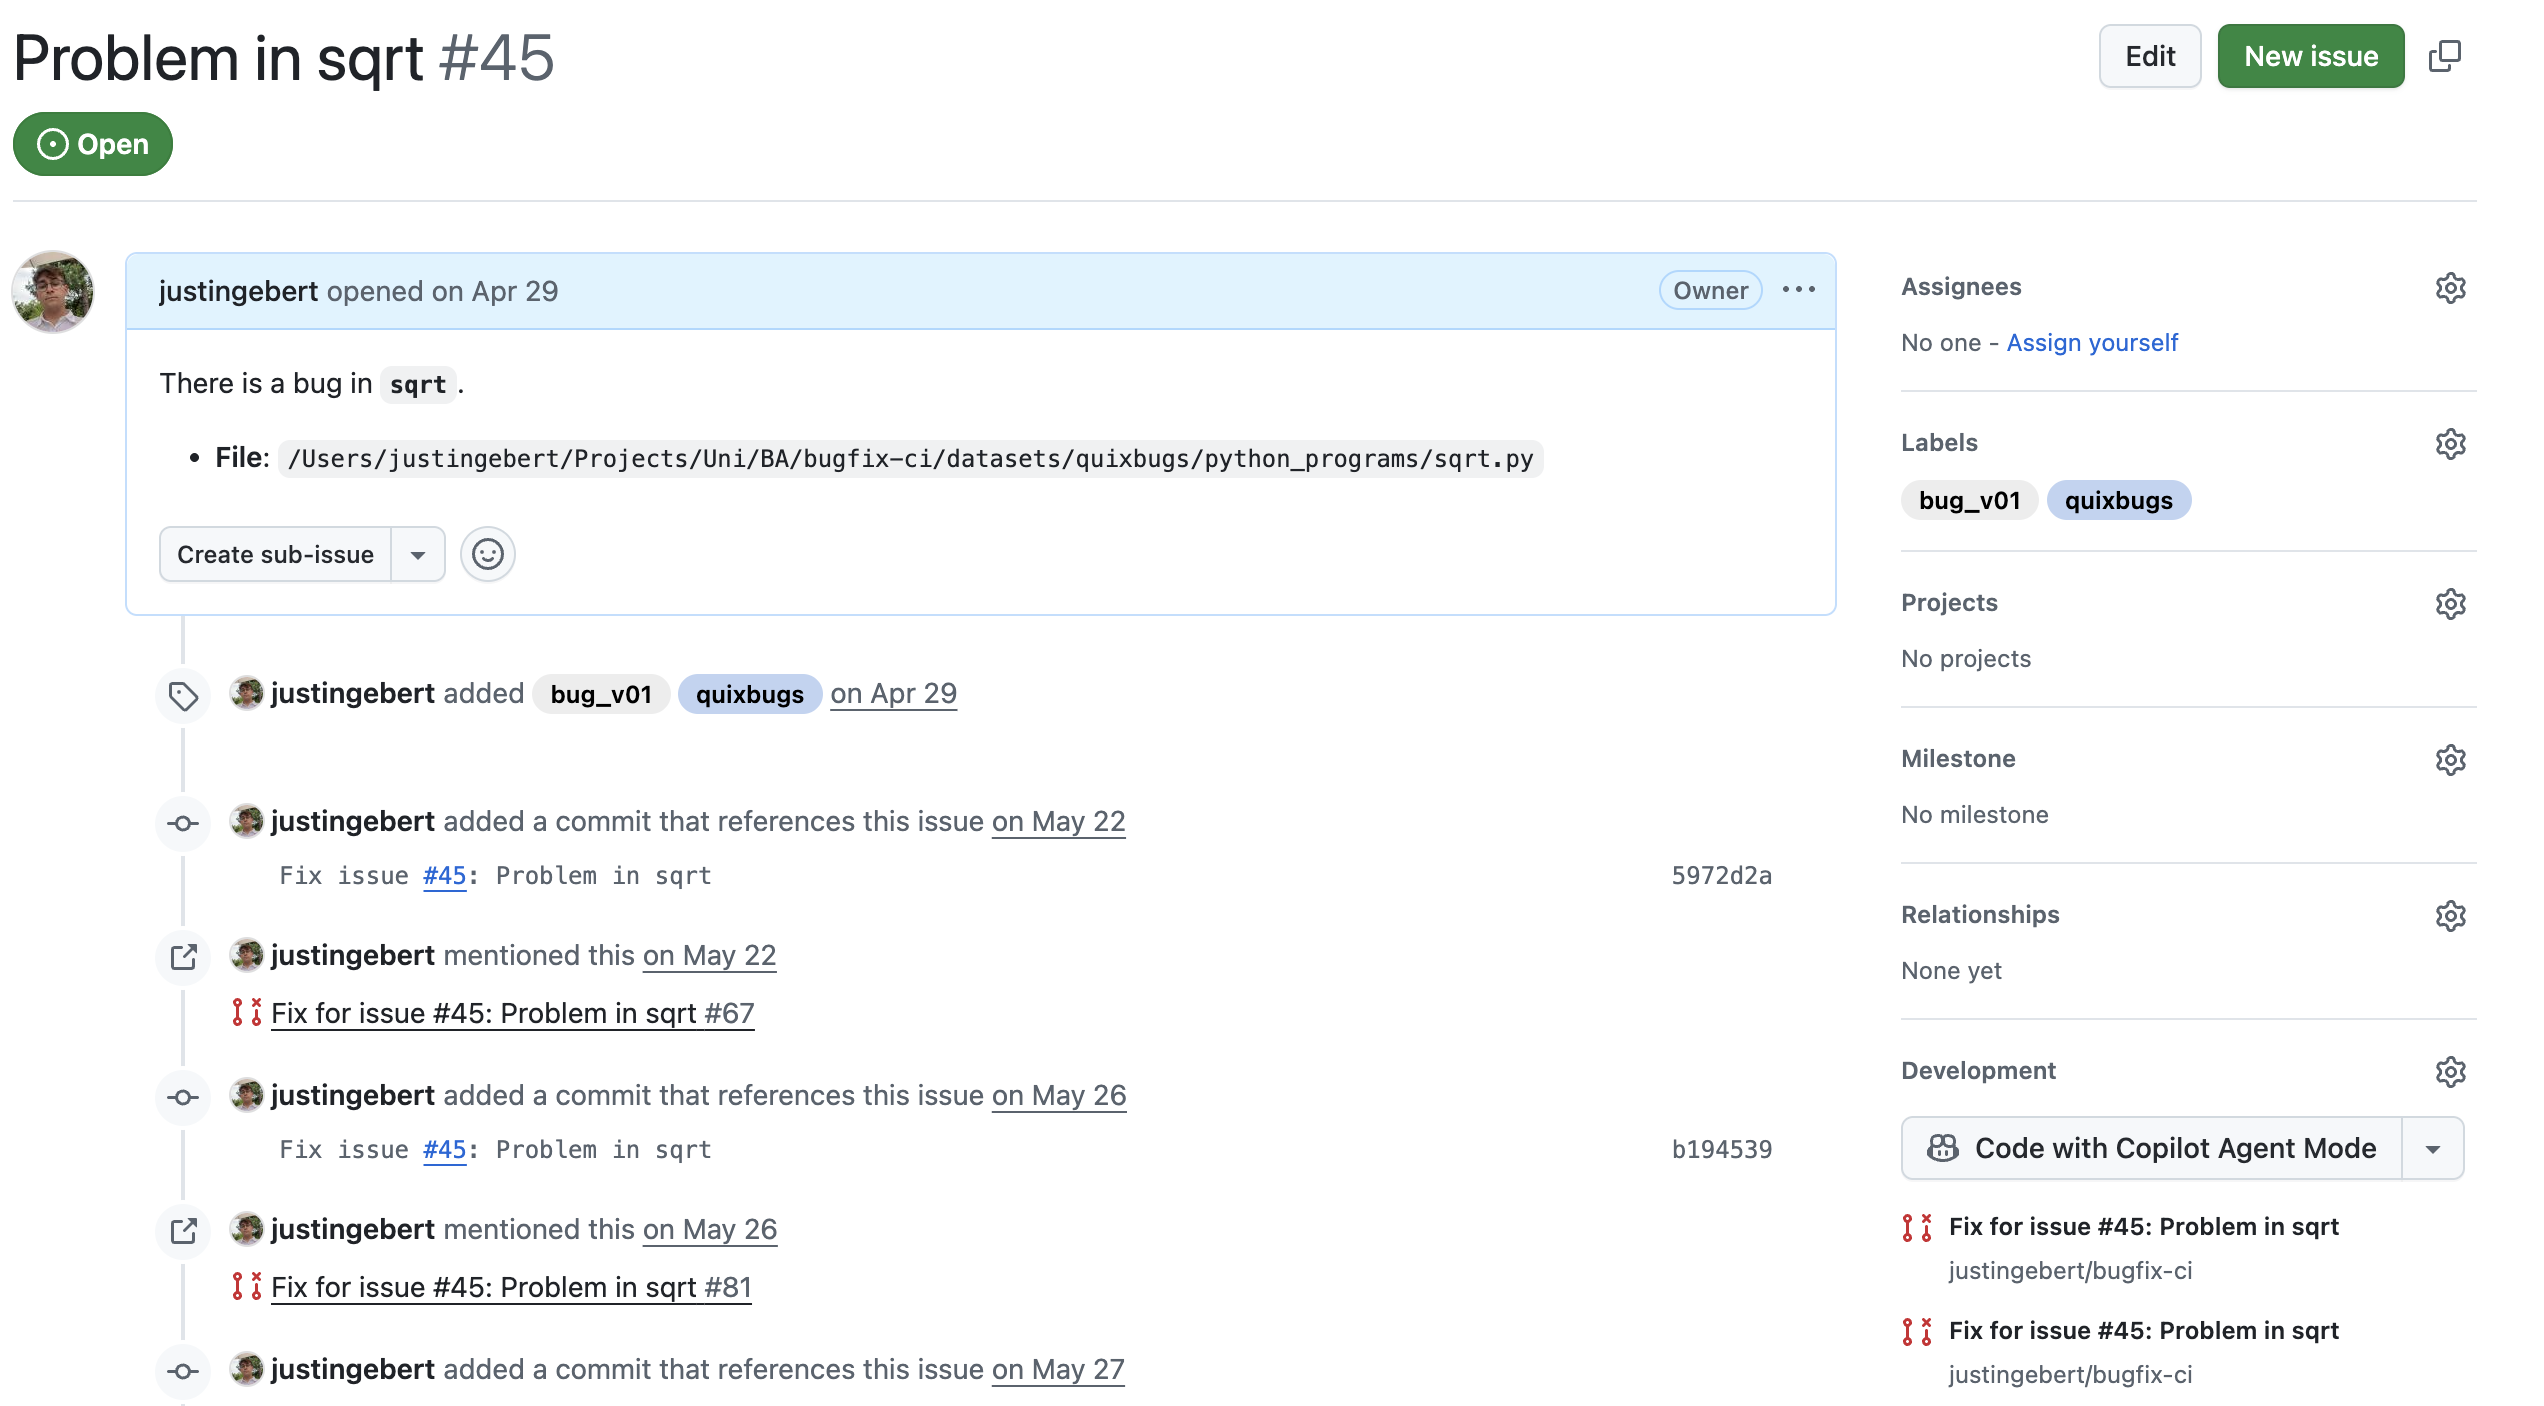
\includegraphics[width=1\textwidth]{images/github/GitHub Issue.png}
    \caption{Example of a GitHub Issue}
    \label{fig:gh-issue2}
\end{figure}

\subsection{Requirements Specification}

Before implementation we constructed the requirements for the prototype following the INVEST model, a widely-adopted methodology in Agile software development \cite{10.5555/984017}. According to the INVEST principles, each requirement was formulated to be independent, negotiable, valuable, estimable, small, and testable. This model ensured that both functional and non-functional requirements were precisely defined, clearly verifiable, and easily adaptable to iterative development and integration within a GitHub-based Continuous Integration pipeline
The requirements are detailed in \ref{chapter:requirements}.
\section{Pipeline Implementation}
The Automated Bug Fixing Pipeline was developed using iterative prototyping and testing, with a focus on simplicity and extendability. Using the self developed requirements \ref{Requirements} we build the following System:

\begin{figure}[H]
    \centering
    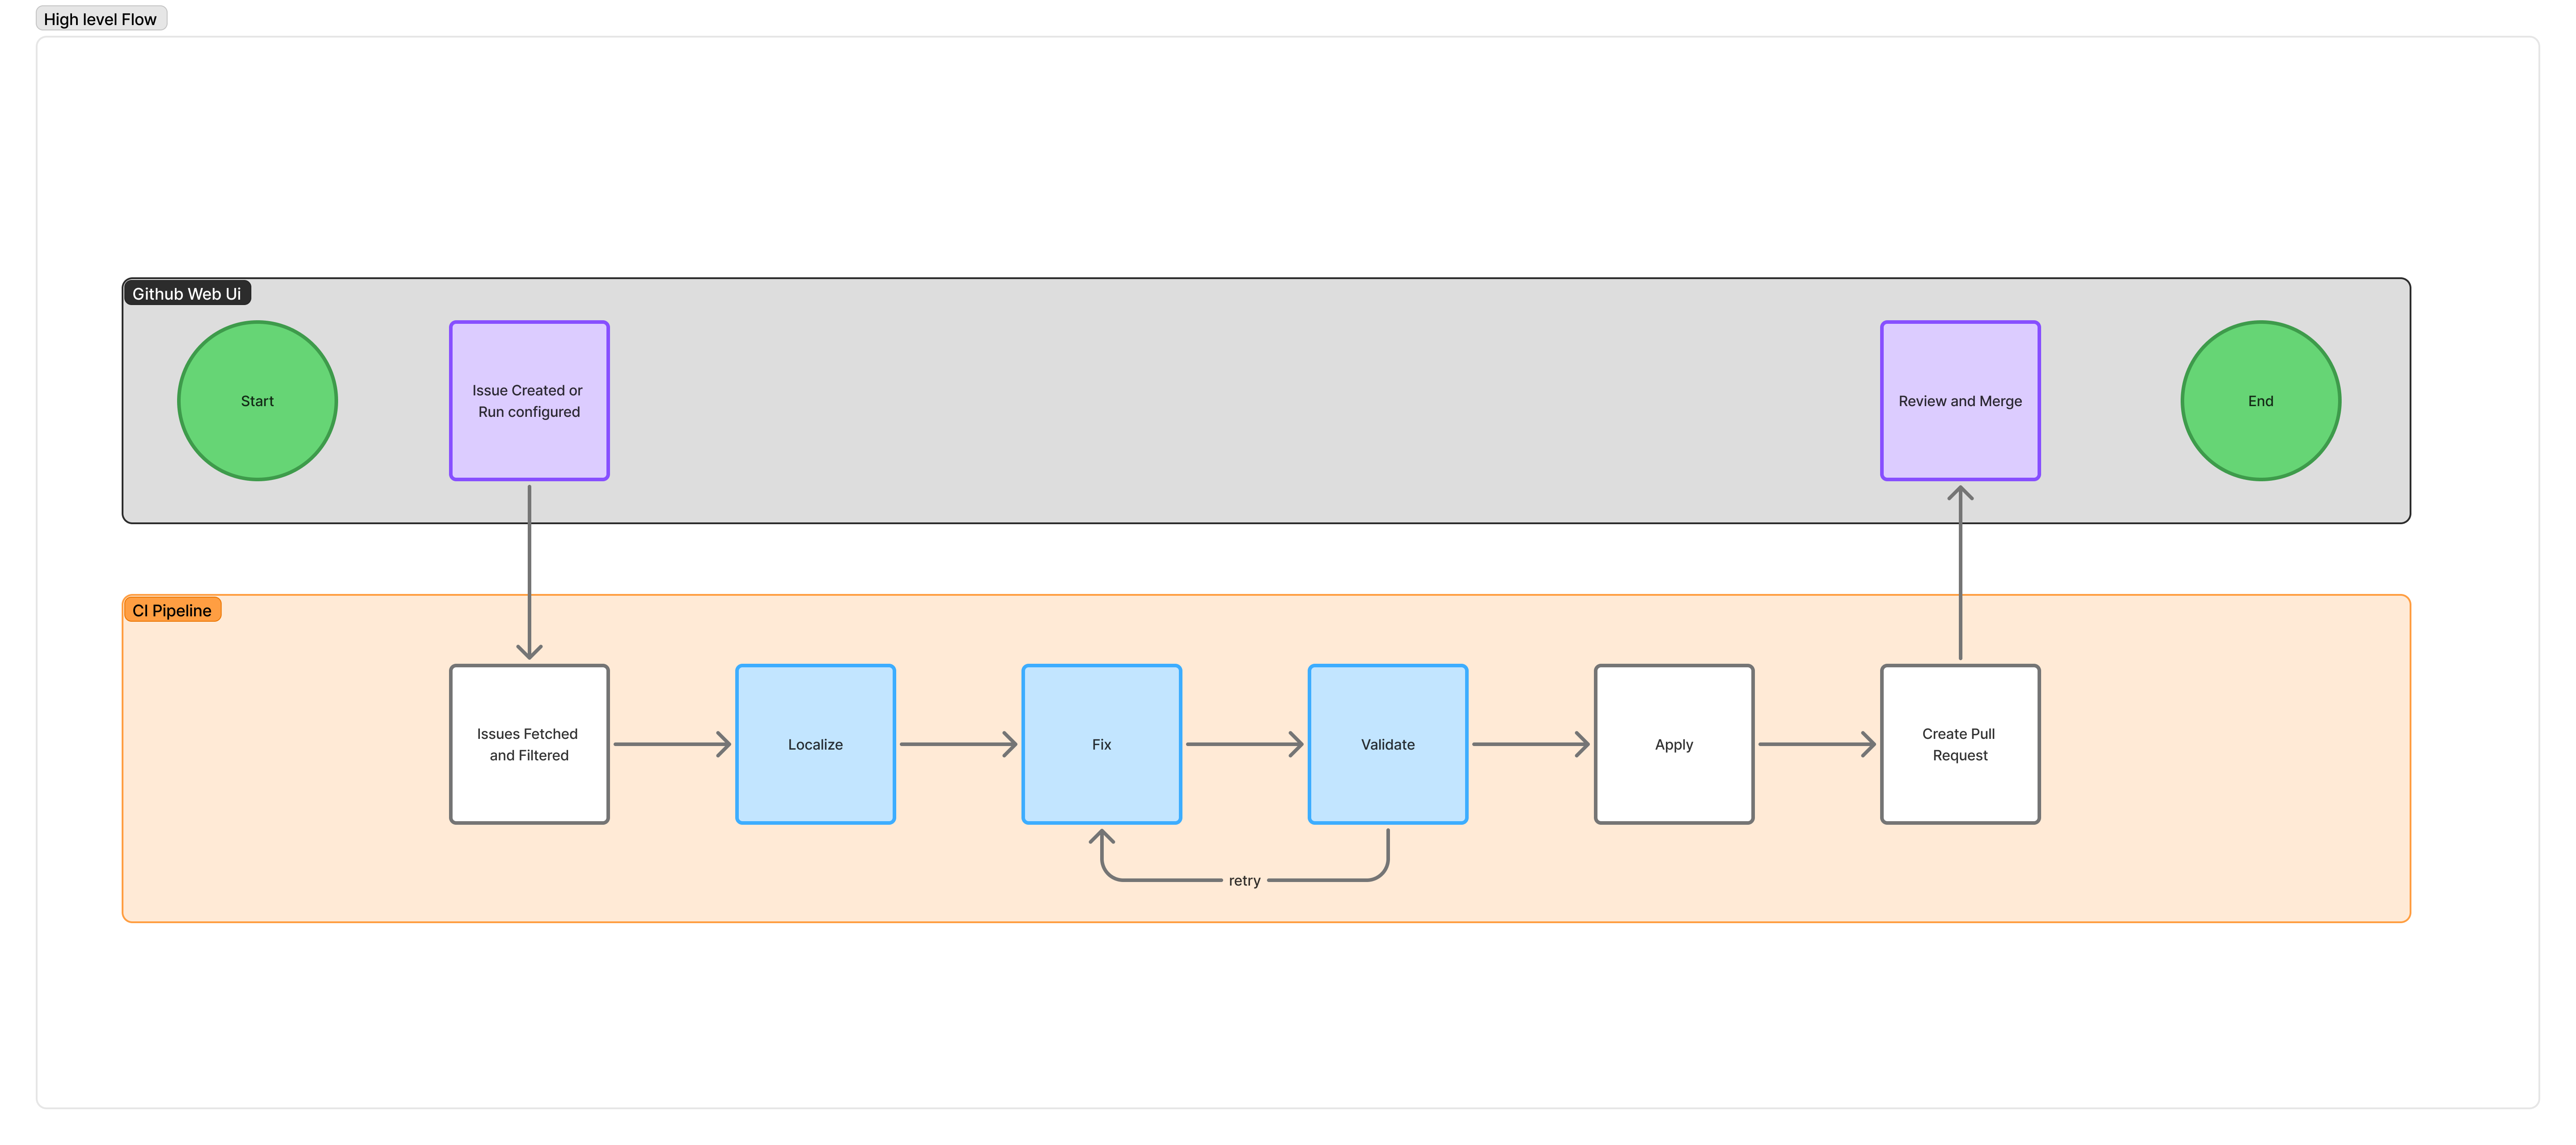
\includegraphics[width=1\textwidth]{images/high-level.png}
    \caption{Continuous Integration Cycle}
    \label{fig:high-level}
\end{figure}

When the system is in place in a target repository. An issue with the default or configured bug label can be created. This trigger trigger will spin up a github action runner which executes the APR pipeline. This Pipeline takes to the configured LLM Api (google and openai) to localize and fix the bugy files. With the supplied file edits the code is validated and tested. When validation passes the a pull request with the file changes is automatically opened on the repository, linking the issue and providing details about the repair process. In case of a unsuccessful repair the failure is reported to the issue.


\section{Evaluation} \label{section:evaluation}

In this section, we describe how we measure the effectiveness and performance of our APR pipeline when integrated into a real-world CI process, using our QuixBugs repository as a bases.

For Evaluation we will focus on several key metrics to assess the system's performance and abilities in repairing software bugs. These metrics will provide insights into the system's efficiency, reliability, and overall impact on the software development lifecycle. The following metrics are automatically collected and calculated for each run of the APR pipeline:

% TODO averages for all bugs on each model and compare single issue runs with multiple issue runs - also for with and without multi attempt and feedback
\begin{itemize}
    \item\textbf{Repair Success Rate:} Calculate the percentage of successfully repaired bugs out of the total number of bugs attempted by using test results.
          A successful repair is defined as a bug passing all tests associated with it.


    \item\textbf{Number of Attempts:} Track the number of attempts made by the system to repair each bug with a maximum of 3 attempts.


    \item\textbf{Overall Execution Time in CI/CD:} Evaluate the time taken for the system to execute within a CI/CD pipeline, providing insights into its performance in real-world development environments.


          % TODO should I split overall execution and stages into separate metrics?
    \item\textbf{Execution Times of Dockerized Agent:} Measure the time taken by the Containerized agent and its stages to execute the repair process and the  execution times of individual stages.

          With this CICD overhead can be calculated and bottlenecks can be identified


    \item\textbf{Token Usage}: Monitor the number of tokens used by the LLM during the repair process, which can help understanding the cost of repairing and issue and the relation between token usage and repair success.


    \item\textbf{Cost per Issue:} Calculate the cost associated with repairing each bug, considering factors such as resource usage, execution time, and any additional overhead.
\end{itemize}

% TODO
explain how these metrics are collected and calculated, including any tools or scripts used to automate the process.
explain how repair success rate is determined

% TODO
ask zhang wether i need to include the evaluation of swe bench lite from the paper or if a ref is enough

% TODO
explain statistical methods used to analyze the collected data, such as averages, medians, and standard deviations. This will help in understanding the variability and reliability of the results.

% TODO 
explain how resuLTS are calculated for model comparison

what I evaluate:
script execution time + CICD overhead
one issue vs multiple issue times
model vs model metrics
costs
attempts vs no attempts in all these categories